\documentclass[12pt,a4paper]{article}
\usepackage[english]{babel} 
\usepackage{csquotes}

\usepackage[%
  backend=biber,
  style=apa,
  natbib=true
]{biblatex}
\addbibresource{refs.bib}
\usepackage{xurl}

\usepackage{hyperref}
\hypersetup{
colorlinks=true,
urlcolor= blue,
citecolor=blue,
linkcolor= blue,
}

\usepackage{graphicx}
\usepackage{subcaption}

% Code to add paragraph numbers and titles
\newif\ifptitle
\newif\ifpnumber
\newcounter{para}
\newcommand\ptitle[1]{\par\refstepcounter{para}
{\ifpnumber{\noindent\textcolor{lightgray}{\textbf{\thepara}}\indent}\fi}
{\ifptitle{\textbf{[{#1}]}}\fi}}

%\ptitletrue  
\pnumbertrue 

% minimum font size for figures
\newcommand{\minfont}{6}

% Allows to rewrite the same title in the supplement
\newcommand{\mytitle}{Identifying contributing factors of train delay through Social Network Analysis}

\title{\mytitle}

\author{Fabian Becker}
\date{\today}

\begin{document}    
    
\maketitle

\begin{abstract}
  Although the German railway network is considered the largest in Europe, it is also infamous for being very unreliable. Since 70 percent of long-distance trains are considered to be not punctual, the German government introduced a railway spending programme with the aim of reducing delays and making the train a more desirable mode of transportation. In order for the spending programme to be successful, it is necessary to identify the factors that cause delays. In this paper, several of these factors will be shown, retrieved from a linear regression analysis. The study revealed that specific train station operators and control centers exert an influence on train delay, both positively and negatively. These insights can be employed to identify optimal train organisation strategies and implement them across the entire network. Furthermore, this research can serve as a foundation for identifying other crucial influences through the utilisation of a larger data set containing more information.
\end{abstract}

\section{\label{sec:Introduction}Introduction}

Germany is home to the largest railway network in Europe, with a total length of over 39,000 kilometers. France is the next largest, with a network of 27,000 kilometers \citep[p.~80]{RailwayLengthStat}. 
However, the railway service in Germany is also known to be chronically unreliable and unpunctual. 
A review of the official data reveals that the punctuality rate of long-distance travelers is approximately 70 percent \citep{dpa2023, DBPunctuality2024}. 
This figure may appear satisfactory at first glance, but it is important to consider that delay in terms of the German Railway Service (Deutsche Bahn, DB) means arriving at least 15 minutes late to your destination.

To provide context, Switzerland, a neighboring country to Germany, has a punctuality rate of 90 percent for long-distance train \citep{SBB2024}. 
The reliability of Deutsche Bahn trains is so poor, that the Swiss Federal Office of Transport proposed to stop German trains from entering too deep into the country in order to prevent cascading delays on their own trains  caused by the DB trains \citep{Magill2023}.

Delay is one of the most significant reasons why the German government introduced a 47 billion euro rail-spending program in order to overhaul the railway network, improve reliability and most importantly to reduce CO\textsubscript{2} emissions by making the train an equally attractive mean of transport \citep{Scally2023}. 
One of the first measures to make traveling by train more appealing was to introduce affordable train tickets in the form of a 49 Euro Ticket \citep{DW2023}, however if German trains lack general punctuality, the reduced travel costs will not necessarily result in a shift in customer preference towards rail travel over private vehicles.

In order to spend this money purposefully, an in-depth analysis of the German railway system is needed in order to determine plausible causes for unreliability and train delay. 
Hence to this event I want to discover if Social Network Analysis is a fitting tool in order to find structural causes for train delay that can only be eliminated by targeted investments. 

In the first part of this paper, I will construct a network from historical delay data, and also gather metadata about the stations that form the network. 
I will then conduct a descriptive analysis of the network, before using linear regression to identify features from the network that may be correlated with train punctuality.

\maketitle
\section{\label{sec:Related Work}Related Work}

The act of predicting train delay has received a lot of a from science over the years, with the primary objective of enhancing customer satisfaction by reducing the unpredictability of travel times. 
Train delay prediction can also assist in more accurately planning the utilization of the train network by train traffic control \citep{Spanninger2022}. 
Despite the fact that this paper does not focus on train delay prediction, determining factors for train delay represent a vital component in the production of precise prediction model.

\cite{Spanninger2022} reviewed and classified a variety of prediction models, into event-driven and data-driven approaches. 
Event-driven model incorporate train-events, such as departure, arrival and pass-through in order to mimic the railway operation dynamics. 
On the other hand data-driven approaches generate their predictions utilizing historic train movement data, most of the models therefore are machine learning models. 
In this paper also relies on historic delay data derived from arrival and departure times whereas it could be classified as a data-driven approach. 

\cite{Cheng90} for example created a delay estimation system based on non linear equations. 
They specifically introduced train timetables as a part of their model instead of assuming that trains are uniformly distributed over time. 
this paper also utilizes timetable data in order to calculate the required delay data.

\cite{Murali2010} created a linear regression model to predict railroad delay. 
However instead of historic train data they generated their training data by using a simulation and later applied the resulting model to subsections of the Los Angeles train network. 
The main part of this paper is also employing linear regression, nevertheless here the aim is find important factors that determine train delays and would therefore assist in the improvement of such a linear regression model.

Another academic paper written by \cite{Hauck2020} makes use of the same linear regression model, however they used a dataset that was provided by the german railway service and is structured in similar fashion to the one that will be constructed as a part of this research. 
The dataset contains timestamps of the excepted events and the actual time of the event to calculate the delay out of the difference. This at first glance seems almost identical to want will be executed in this paper, however the mentioned research was again only interested in providing an accurate prediction system.

Research that aims to determine factors that cause train delay has been conducted by \cite{Dingler2010}. The goal of this paper was gain a better understanding for delay-causing factors. 
They obtained their data from a railway simulation software and observed the relationship of delay and factors such as train volume or train speed.

This overview of related works helps to draw the conclusion, that the topic of train delays as quite recognized in science.
Hence this paper embeds ideas that have already been observed in different perspectives. 
But ultimately the application of Social Network Analysis on historic german railway data in order to observe possible factors of train delay is an idea that has been absent from research until now.  

\maketitle
\section{\label{sec:Dataset}The dataset}

The most time-consuming aspect of this research was the creation of a realistic delay data set. 
In this chapter I will review the data gathering and prepossessing, as well as providing a description of the obtained dataset by using methodology from Social Network Analysis.

\maketitle
\subsection{\label{sec:Gathering}Data gathering}

The first challenge was to obtain historical delay data for German trains. This was complicated by the fact that, unlike many other rail services, Deutsche Bahn does not provide open access to this data \citep[p.~5]{Spanninger2022}. 
Instead, only delay data for the previous eight hours could be retrieved from the official API. 
In order to obtain an acceptable amount of data, regular queries would have to be made over a period of months. This was not possible due to the time constraints of this research. 
However, the necessary data could be found on the Website \href{https://www.zugfinder.net/en/start}{Zugfinder}. This service provides historical delay data for up to two years if a subscription is purchased. 
The delay data is taken from the public timetable of trains and should therefore be as accurate as the official data. However, it only collects data for long-distance trains, unlike the official API, which also provides information on regional trains. 
For the purpose of this research, however, the available data is sufficient as regional trains have a punctuality rate of over 90 percent compared to around 70 percent for long-distance trains \citep{DBPunctuality2024}. 
As the site does not provide an API by default, a web scraper was written to collect a reasonable amount of data. The resulting source code is available on my personal GitHub repository \citep{repo}. 

In order to gather the requisite data, I initially retrieved a list of all German train stations from the official Deutsche Bahn API. 
I then proceeded to remove all stations that do not accommodate trains. Furthermore, I collected metadata, which can be seen in Fig. 1 (build table). 
This data will later be used to determine possible dependencies on various forms of delay. With this list I searched through every departure board on \href{https://www.zugfinder.net/en/start}{Zugfinder}, utilizing the Selenium library in Python, with the goal of finding possible trains to retrieve timetable data from. 
This list was then searched through every departure board on zugfinder.net, utilising the Selenium library in Python, with the goal of finding possible trains to retrieve timetable data from. 
All trains were then processed in order to remove trains that partly operate outside of Germany, as no sufficient metadata was available for the later analysis. 

Subsequently, I compiled the timetable for each train of the previous two months. This data then was processed in order to calculate the delay rates of the trains utilizing the contained arrival and departure times at every given stop.

\maketitle
\subsection{\label{sec:Preprocessing}Data preprocessing}

The obtained data was then preprocessed by again checking for possible non german train stops inside of the timetables. This happens due to the fact, that train lines can serve as a replacement train on lines that also operate outside of Germany. Next the remaining data was used to calculate various metrics necessary for later inspection (Fig2.). Moreover canceled stops were also removed. 
The list of possible stations retrieved earlier also needed to be updated, all stops that are not a part of the processed train data. Finally the network consists of 305 train stations that function as nodes and 1389 directed edges. The edges were constructed from the available timetable data.

\maketitle
\subsection{\label{sec:Preprocessing}Description of the dataset}

The final network comprises 305 train stations that function as nodes and 1389 directed edges. The edges were constructed from the available timetable data and are visualised in Figure~\ref{fig:network-map} using the provided geodata via the Matplotlib Basemap package.

\begin{figure}[h]
  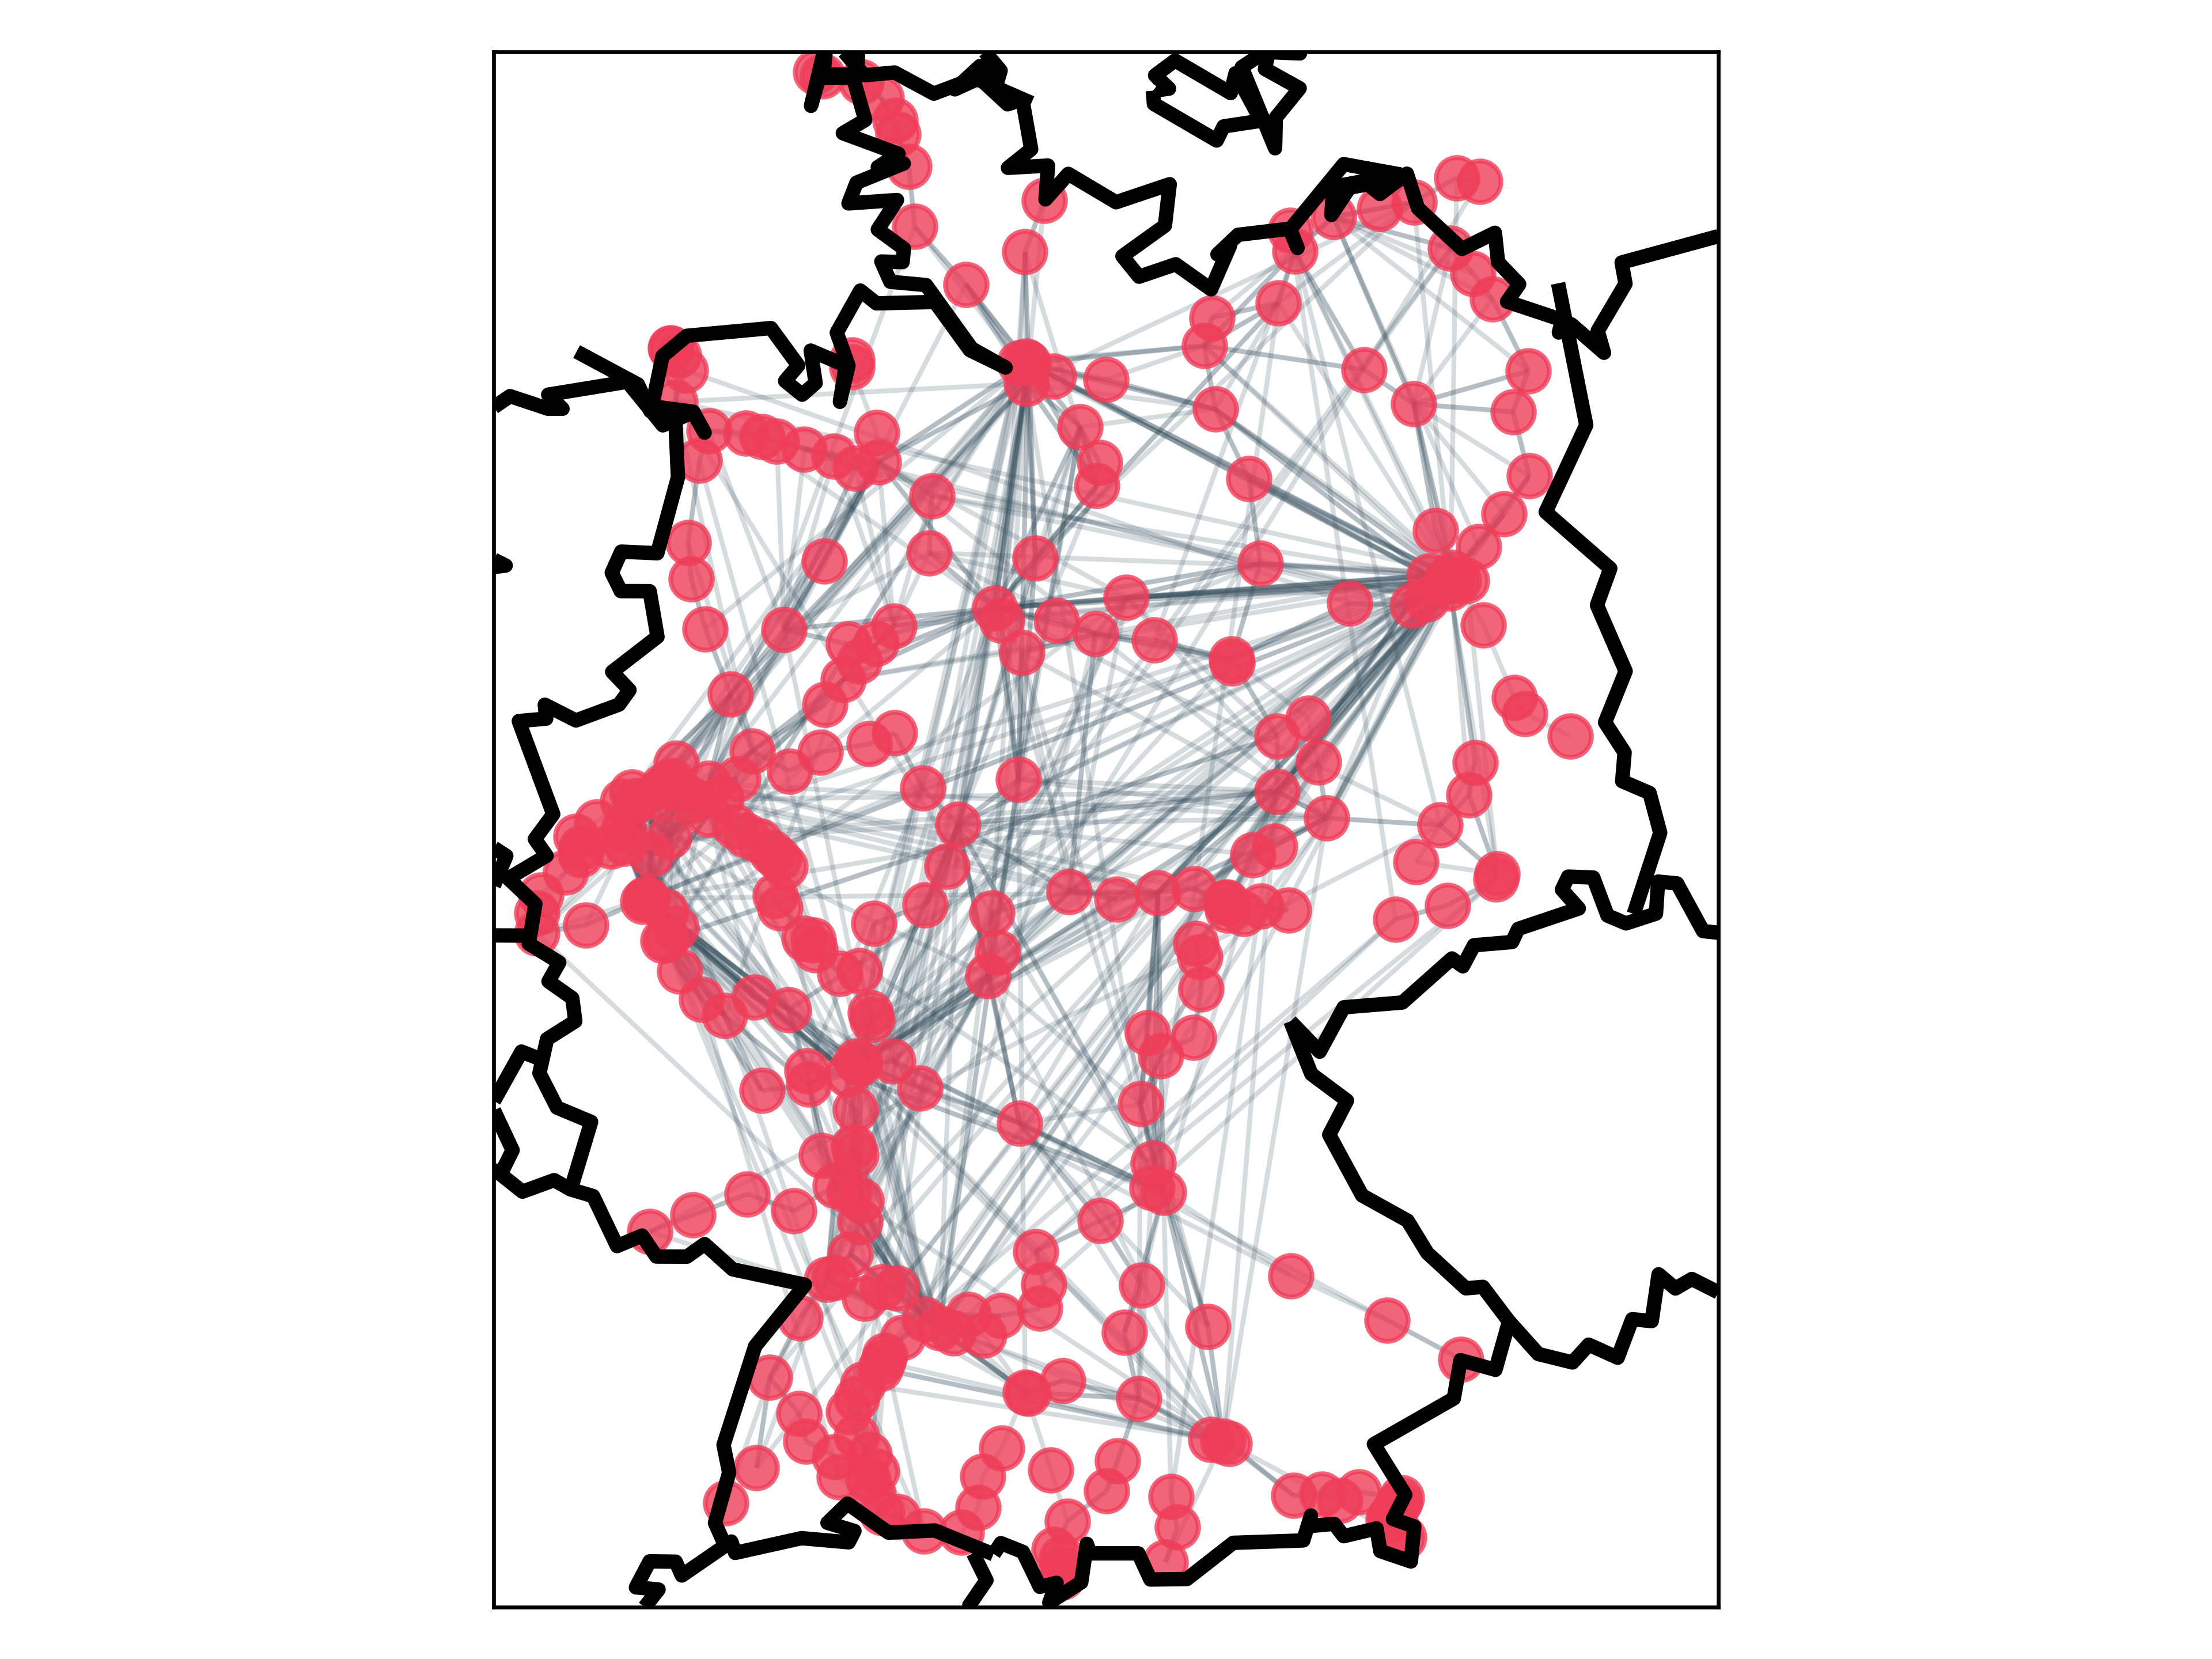
\includegraphics[clip=true,width=\columnwidth]{../data/visualizations/network.png}
  \caption{The obtained network visualized on the German map}
   \label{fig:network-map}
\end{figure}

In this network model, the nodes are the individual train stations, and the corresponding directed edges are the connections between different train stations used by at least one train. 

\begin{table}[]
  \centering
  \begin{tabular}{lllll}
  \hline
                 & \textbf{Metropolitan} & \textbf{Interchange} & \textbf{Feeder} &  \\ \hline
  amount         & 18                                    & 202                          & 83                              &  \\
  share     & 6 percent                             & 67 percent                   & 27 percent                      &  \\
  average platforms     & 16                            & 6                   & 3                 &  \\
  average degree & 30.39                                 & 9.17                         & 4.54                            &  \\ \hline
  \end{tabular}
  \caption{Different nodes types, their share, average degree and platforms}
   \label{fig:network-overview}
\end{table}

Table~\ref{fig:network-overview} depicts that the nodes in the network can be separated into three main types of stations.

\begin{itemize}
  \item Metropolitan railway stations are located in larger cities and handle a substantial amount of train traffic. 
  Consequently, a high number of trains arrive and depart from these stations, resulting in a disproportionately high average degree.
  \item It can be observed that interchange stations are considerably smaller than other types of stations, as evidenced by the number of platforms. They account for over two-thirds of the network's nodes. The average degree of interchange stations is almost identical to the degree of the general graph and is considerably higher than what would be assumed in a train station network. This is due to the fact that the underlying dataset only consists of long-distance trains.
  \item Feeder stations are smaller stations situated in more rural areas. Their primary function is to facilitate the connection of passengers to larger railway stations, enabling them to embark on their desired long-distance trains. Nevertheless, it is evident that some long-distance trains include these stations in their schedules.
\end{itemize}

The findings of the network are comparable to the Barabasi Albert Model of preferential attachment. This can be observed in the degree distribution of the network. 
Figure~\ref{fig:network-deg-dist} does not show a perfect power law distribution, as can be validated by Figure~\ref{fig:network-powerlaw}. 
However, the Metropolitan railway stations function as a target for preferential attachment, which is logical given that smaller train stations connect to larger ones to facilitate passenger access to as many destinations as possible. 
Nevertheless, this also introduces potential reasons for delay, as larger train stations may not be able to accommodate the influx of incoming trains effectively, potentially due to a lack of platforms. Alternatively, connections to the Metropolitan stations may be congested by the sheer number of trains utilizing them, which in turn results in cascading delays. 
Therefore, the hypothesis will be examined in greater detail at a later stage. 

The network in general is also notably sparse, as evidenced by the edge density of approximately 0.015. 
A dyad census yielded 44,800 unlinked nodes, 435 mutually connected nodes, and 518 asymmetric nodes. 
The aforementioned findings can be attributed to the nature of the dataset. The data utilized in this study originates from long-distance railways, necessitating the use of well-developed tracks to enable the trains to operate at high speeds. Given the higher maintenance requirements of these tracks, alternative routes are rarely provided.

\begin{figure}[h]
  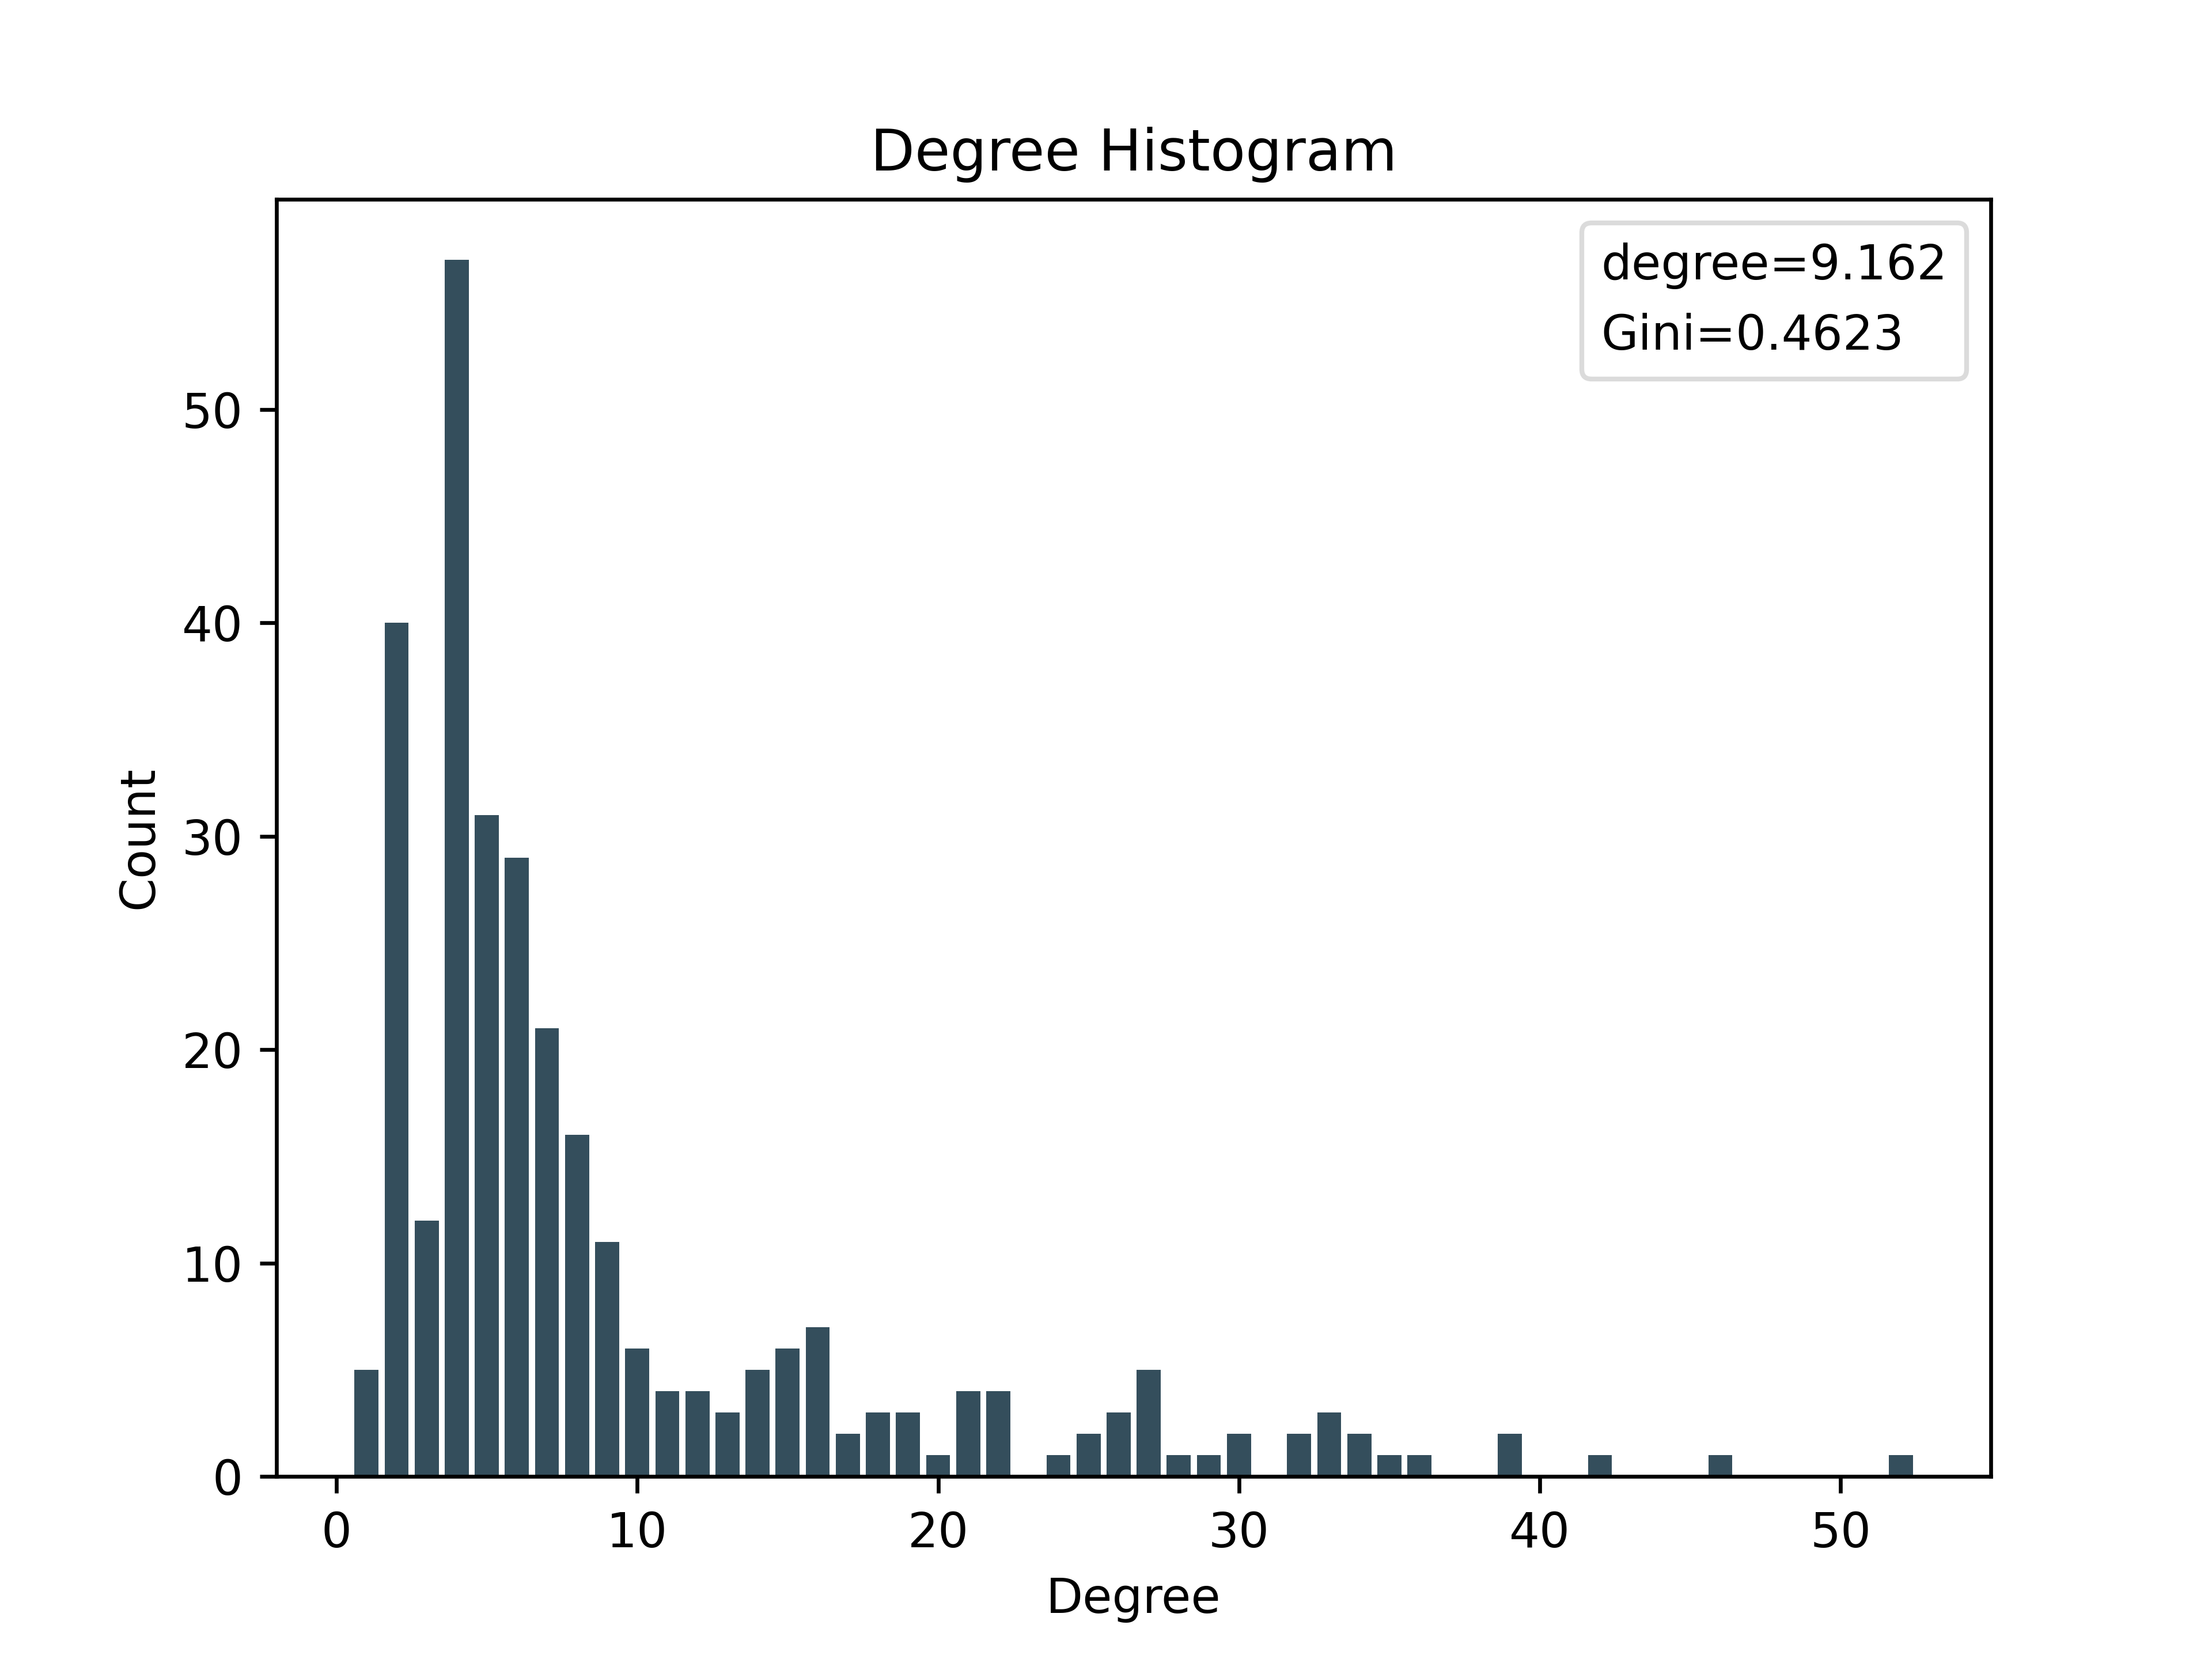
\includegraphics[clip=true,width=\columnwidth]{../data/visualizations/degree_dist.png}
  \caption{The degree distribution of the network}
   \label{fig:network-deg-dist}
\end{figure}

\begin{figure}[h]
  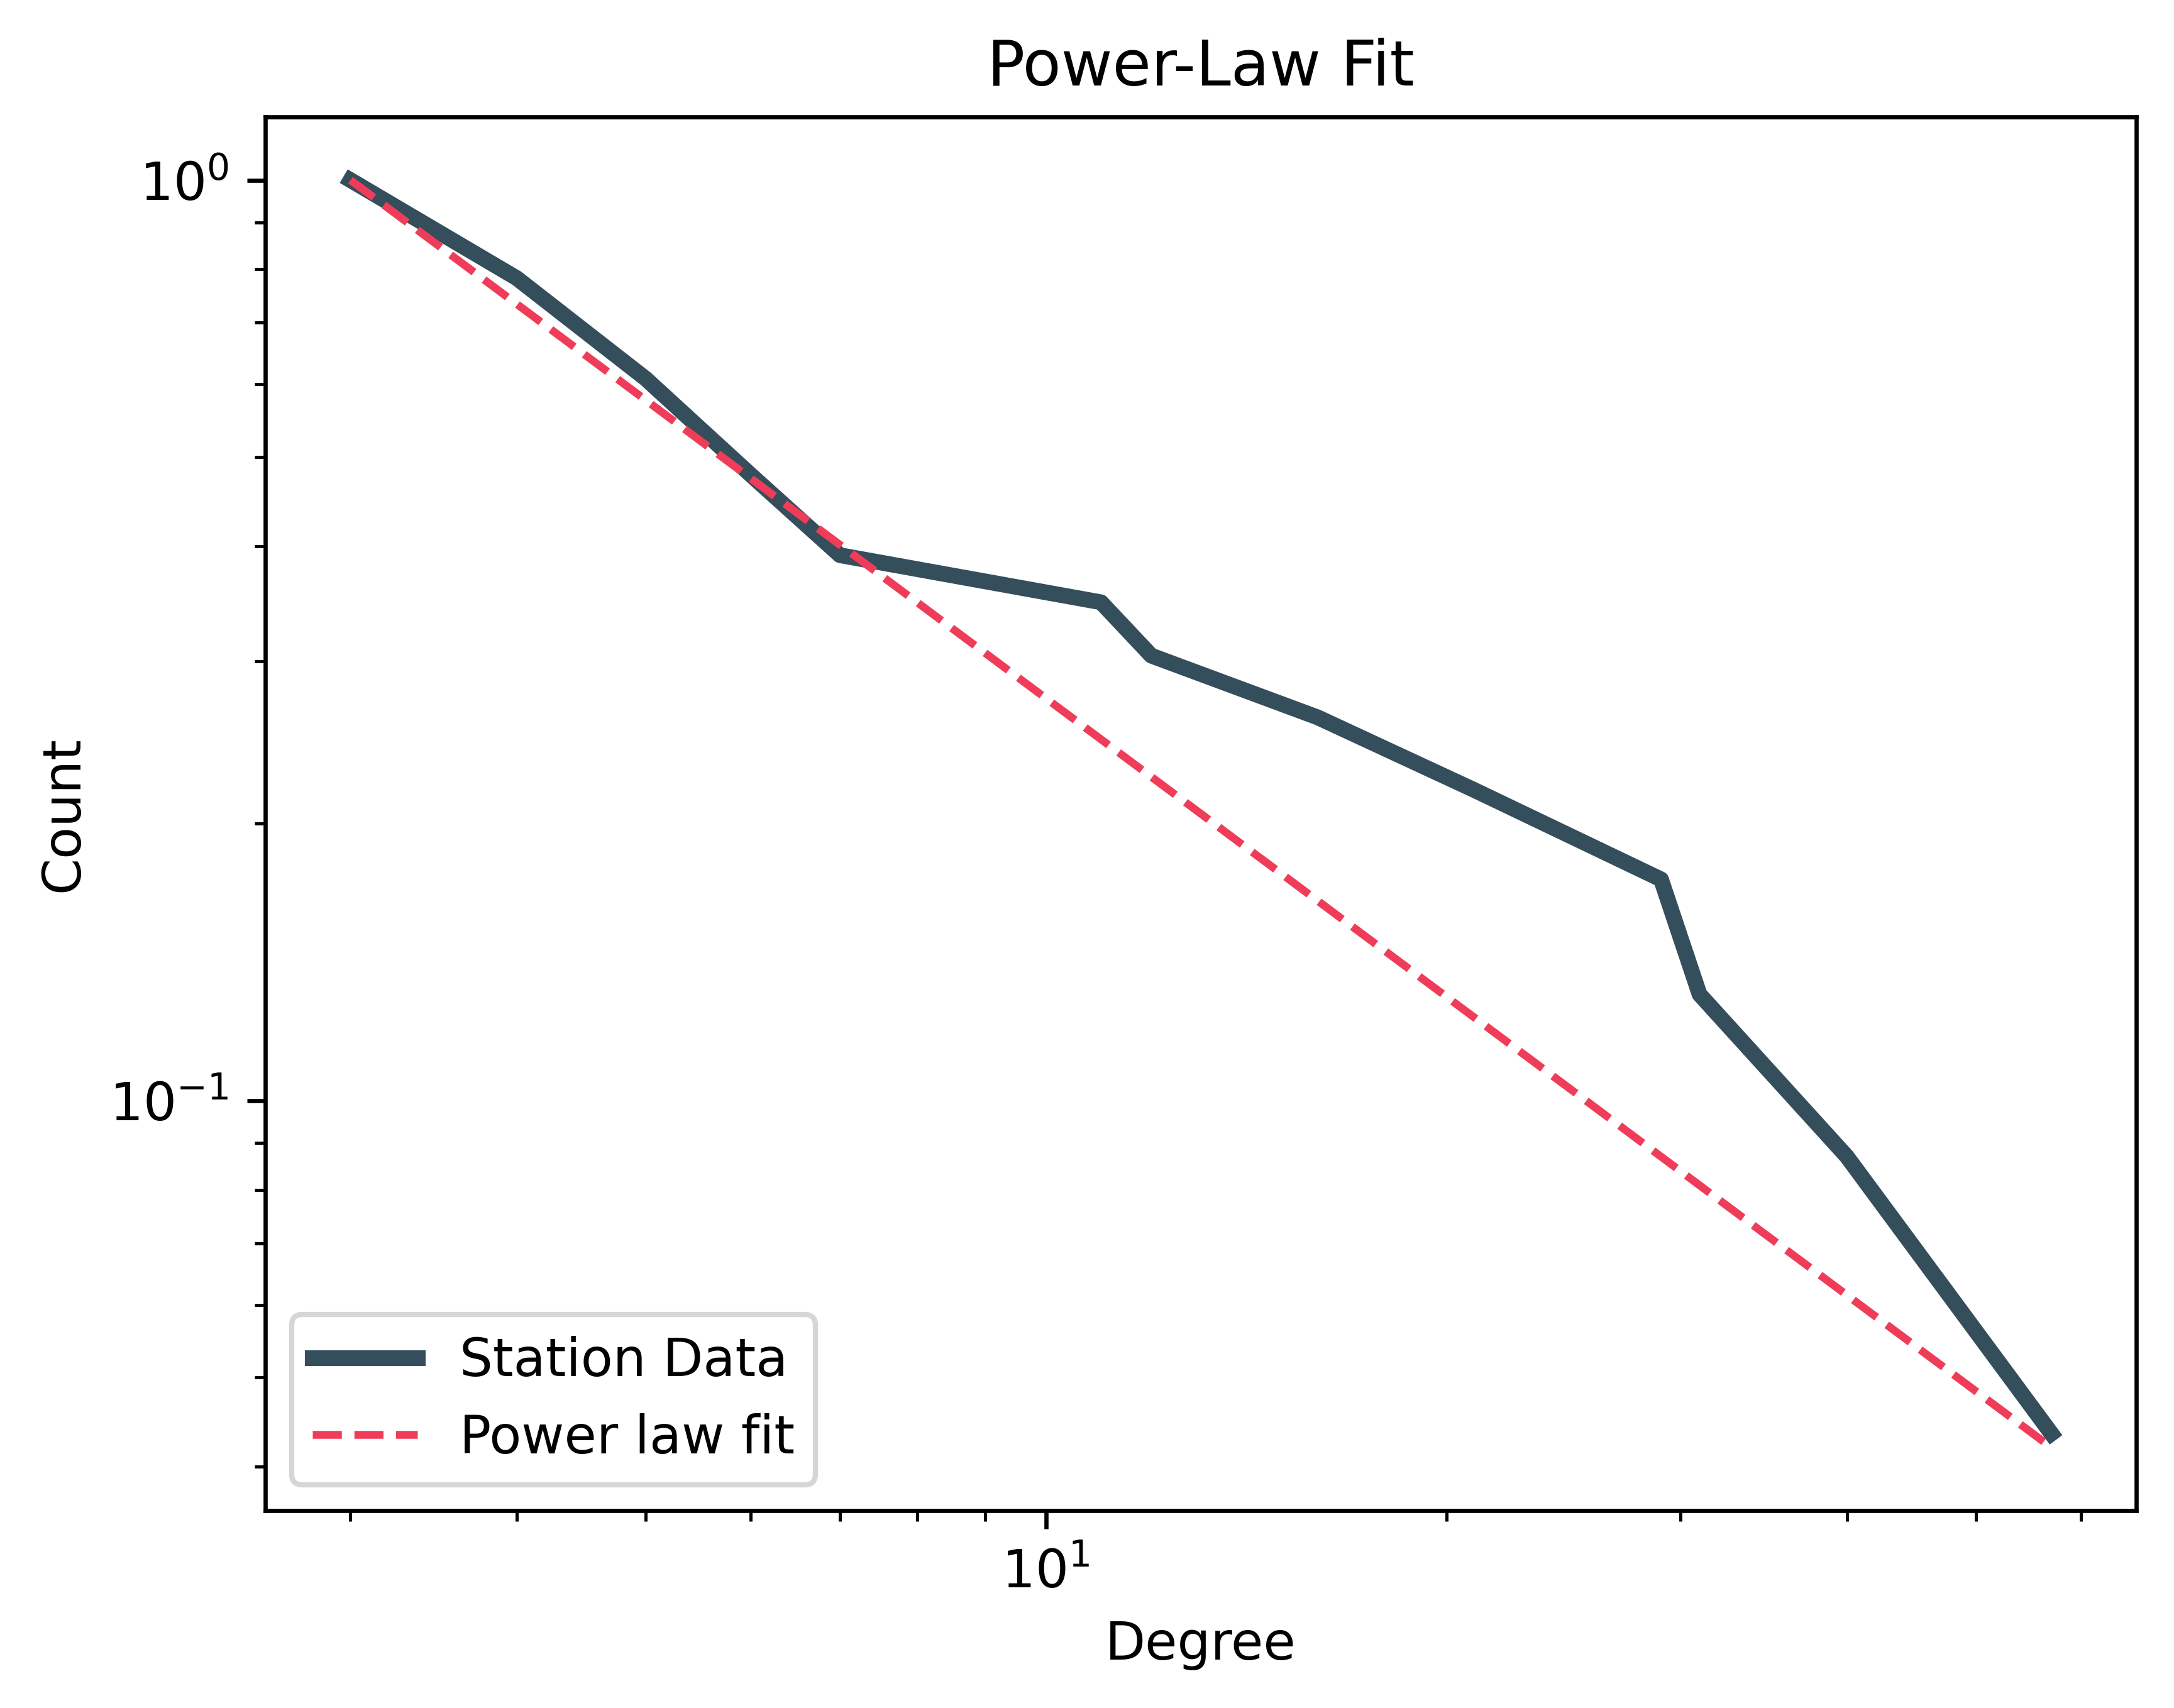
\includegraphics[clip=true,width=\columnwidth]{../data/visualizations/powerlaw_fit.png}
  \caption{Power-law fit of the obtained degree distribution}
   \label{fig:network-powerlaw}
\end{figure}

Nevertheless, the maximum distance of the network is relatively short, with the shortest path from Berchtesgaden, which is in close proximity to the Austrian border in Bavaria, to Klanxbüll, situated in the vicinity of the Danish border, being only 24 edges in length. 
It can be concluded that the presence of a passing node does not necessarily indicate the necessity for a train switch, which implies that every destination in this network is quite reachable. The reciprocity is also quite high at approximately 0.627, which can be interpreted as follows: If one were to travel to a particular destination via a specific number of stations, it is likely that a similar route exists which would allow one to return to their original point of departure. 

Upon initial observation, the infrastructure of the German long-distance train appears to be well-designed and free of significant design flaws. Nevertheless, the network exhibits a lack of reliability, necessitating the use of linear regression to examine potential dependencies in greater depth.
\maketitle
\section{\label{sec:Research methodology}Research methodology}

This chapter is devoted to the research question of this paper. Linear Regression will be used to determine possible dependencies of train delay inside the network, this method is a simple technique of predicting a variable $Y$ from one or more predictor variables $X$, assuming that there is a linear relationship between those variables \citep[p.~70]{James2023}. 
In this part, we will attempt to identify suitable predictor variables from metrics obtained through social network analysis and metadata contained within the network.

The predicted variable $Y$ is also populated with different choices throughout the experiments. Initially, both values for stations and for connections are present in order to identify relevant factors on both of them. 
Furthermore, stations have values for both incoming and outgoing delay properties in order to detect possible reasons in more detail. Finally, two different kinds of delay metrics are employed: the average delay and the standard deviation. 
The average delay denotes the average delay of all trains in order to capture the general idea of delay. Conversely, the standard deviation should reflect the overall reliability of the delay, given that reliability is also a significant factor for travelers. 
For instance, if a train is consistently five minutes late, the timetable can be adjusted accordingly. However, if the train is on time on some days but experiences significant delays on others, this can significantly impact traveler comfort and potentially result in passengers missing connecting trains.

For computing metrics on the network, the Python library \href{https://networkx.org/}{NetworkX} was employed. The linear regression was executed using the R programming language, with the \href{https://cran.r-project.org/web/packages/olsrr/index.html}{Oslrr} Package used to facilitate the identification of suitable regression variables.

\maketitle
\section{\label{sec:RealtionshipCentrality}Exploring the relationship of centrality measures and delay}


As previously stated in Chapter \ref{sec:Research methodology}, the centrality of a train station or a connection may influence the delay. The simplest measure of this is the degree, which simply counts the adjacent nodes. Since the data provides directed edges, the degree is separated into in-degree and out-degree. 

Testing the average incoming delay and average outgoing delay on their linkage to the incoming and outgoing degree does not reveal a meaningful connection. Firstly, the in- and outdegree are highly linearly dependent and therefore cannot both be used as predictor variables at the same time. This is a predictable result, given that only two stations on each train ride function as starting or end station, where the degree differs. Even if a model is constructed with one of the directed degrees, the p-value of all four combinations is between 0.003 and 0.004, which is a relatively high value. Furthermore, the adjusted R² error is only around 0.01, indicating that these models do not cover a significant range of variations. Despite this, all four models show a slight positive correlation between average delay and degree, suggesting that further exploration of the hypothesis is warranted. The model indicates that the average delay is higher at stations with a greater number of connections to other stations. Since the edges merely describe different connections and do not provide information about the utilisation of the latter, the number of handled trains was added in order to potentially improve the model. However, both of the predictors are again highly collinear, and therefore the given model is not reliable.

On the other hand, the correlation of degree and the standard deviation of the delay provides much more promising results. The models exhibit a very low p-value, while the adjusted R² error is approximately 0.7 for all combinations. Furthermore, the model depicts a positive relationship between degree and standard deviation, with an estimated value of approximately 8. This leads to the conclusion that at stations with higher degrees, trains arrive and depart less reliably. 

The betweenness centrality incorporates information about the brokerage of a particular node and therefore the shortest path connecting two railway stations \citep[p.~35]{Linton}. This centrality measure will be the starting point of the next linear regression model. It is unfortunate that the average delay of a station based on the betweenness centrality generates worse results than the model with degree centrality. The application of betweenness centrality to the standard deviation again signals a positive relationship, with the model exhibiting a very low p-value. Conversely, the adjusted R² is somewhat lower this time. As betweenness centrality can also be calculated for edges, this model was also explored. Unfortunately, this model did not yield any new insights. 

The closeness centrality, which incorporates the notion of proximity between nodes \citep[p.~180]{Rodrigues2019}, has also been examined. However, the model did not yield any novel insights.

\maketitle
\section{\label{sec:RealtionshipMeta}Exploring the relationship between the collected metadata and delay}

During the data gathering process, additional metadata was collected with the objective of detecting other potential influences on the delay. 
This chapter will examine the possible variables that may have contributed to the observed phenomenon.

First the number of platforms at a particular railway station is initially considered as a potential predictor variable. The resulting linear model exhibits a p-value that is close to zero, thereby providing insights that are of considerable value. The average delay is once again found to have a positive correlation with the number of platforms. The same results can be observed when the average delay is replaced by the standard deviation as a prediction result. One possible explanation for this phenomenon is that railway stations with a larger number of platforms are more difficult to manage.
This is supported by the fact that nine of the ten railway stations with the most number of platforms are Metropolitan stations.

Previous models have indicated that metropolitan stations experience higher delays due to their higher degrees and larger number of platforms. This study examines the type of station as a potential predictor variable. The model actually proves this hypothesis. In contrast to the positive correlation between Metropolitan stations and average delay, Feeder railway stations have a negative influence on delay. 
This observation is consistent with the results of previous models, since these stations in general have fewer platforms and a low degree, as illustrated in Table~\ref{fig:network-overview}.

The metadata collected also includes information about the station operators. By constructing a model that uses this data, it is possible to identify which operators are able to coordinate their stations efficiently. Using the operator as a single predictor variable creates interesting output. 
Firstly, the p-value for most operators is too high to draw any applicable conclusions from the data. 
However, for two station operators, the p-values are sufficient. 

The operator \textit{Nahverkehrsgesellschaft-Baden-Württemberg-MBH} has the second lowest p-value and a negative correlation of -3 with the average delay. 
Given that the mean of the average delay across the entire dataset is approximately 5.975, it can be concluded that the operator is performing extremely well. 
In order to ascertain the potential reasons for this performance, the number of operated stations was initially examined, as a low number of operated stations may be more easily managed. 
However, the operator from Baden-Württemberg actually operates 47 stations, which is equal to the operator from Bavaria and the highest amount in the dataset. 
One might then hypothesise that this particular station operator does not manage any metropolitan stations, given that the previous observations indicated that metropolitan railway stations tend to result in higher average delays. 
However, this hypothesis is also found to be incorrect, as this operator manages 16.6 percent of all metropolitan stations. 
In order to identify a potential explanation for this exceptional punctuality, it is necessary to conduct a review of Chapter~\ref{sec:Introduction}. 
Baden-Württemberg is situated in close proximity to the Swiss border. As the Swiss railway operator does not permit delays, the German trains also potentially crossing over to Switzerland require a precise schedule. 
It is important to note that trains that traverse other countries than Germany have been excluded from the railway network. This is because the railway network is an interdependent structure, and therefore, delayed trains in the network of Baden-Württemberg would also exert influence on trains crossing the Swiss border.

The second most significant p-value belongs to the operator \textit{Verkehrsgesellschaft Mecklenburg-Vorpommern-MBH}, which exhibits a more pronounced negative correlation with delay. 
The estimated value is -6.5. Despite operating at 17 stations, this operator still ranks fifth in the network in terms of the number of stations it serves. 
Conversely, this operator does not manage any metropolitan stations, which may account for this performance. 
Furthermore, the federal state of Mecklenburg-Vorpommern has only one international border with Poland, in contrast to Baden-Württemberg, which has multiple international borders. 
This results in less international train traffic to be managed in Mecklenburg-Vorpommern. However, this result reinforces the hypothesis that metropolitan train stations in general have a positive effect on delay.

As previously indicated in Table~\ref{fig:network-overview}, the data relating to the control center of each railway station included in the study were also provided.
As with the regression model that employed the operator as a predictor variable, a model that utilized the control center as a predictor variable also yielded a noteworthy insight.
The resulting model yielded a single statistically significant p-value for the control center at the main station in Nuremberg, Bavaria.
This particular station exhibited a highly positive correlation with the average delay, with an estimated value of 5.710. 
One possible explanation for this result is the geographical distribution of the stations. 
As is evident from Figure~\ref{fig:nb-control}, the controlled railway station is distributed over a considerable distance. 

\begin{figure}[h]
  \includegraphics[clip=true,width=\columnwidth]{../data/visualizations/Nürnberg_controlled_stations.png}
  \caption{Visualization of the train stations controlled by Nürnberg main station, which is colored in red}
   \label{fig:nb-control}
\end{figure}

\begin{figure}[h]
  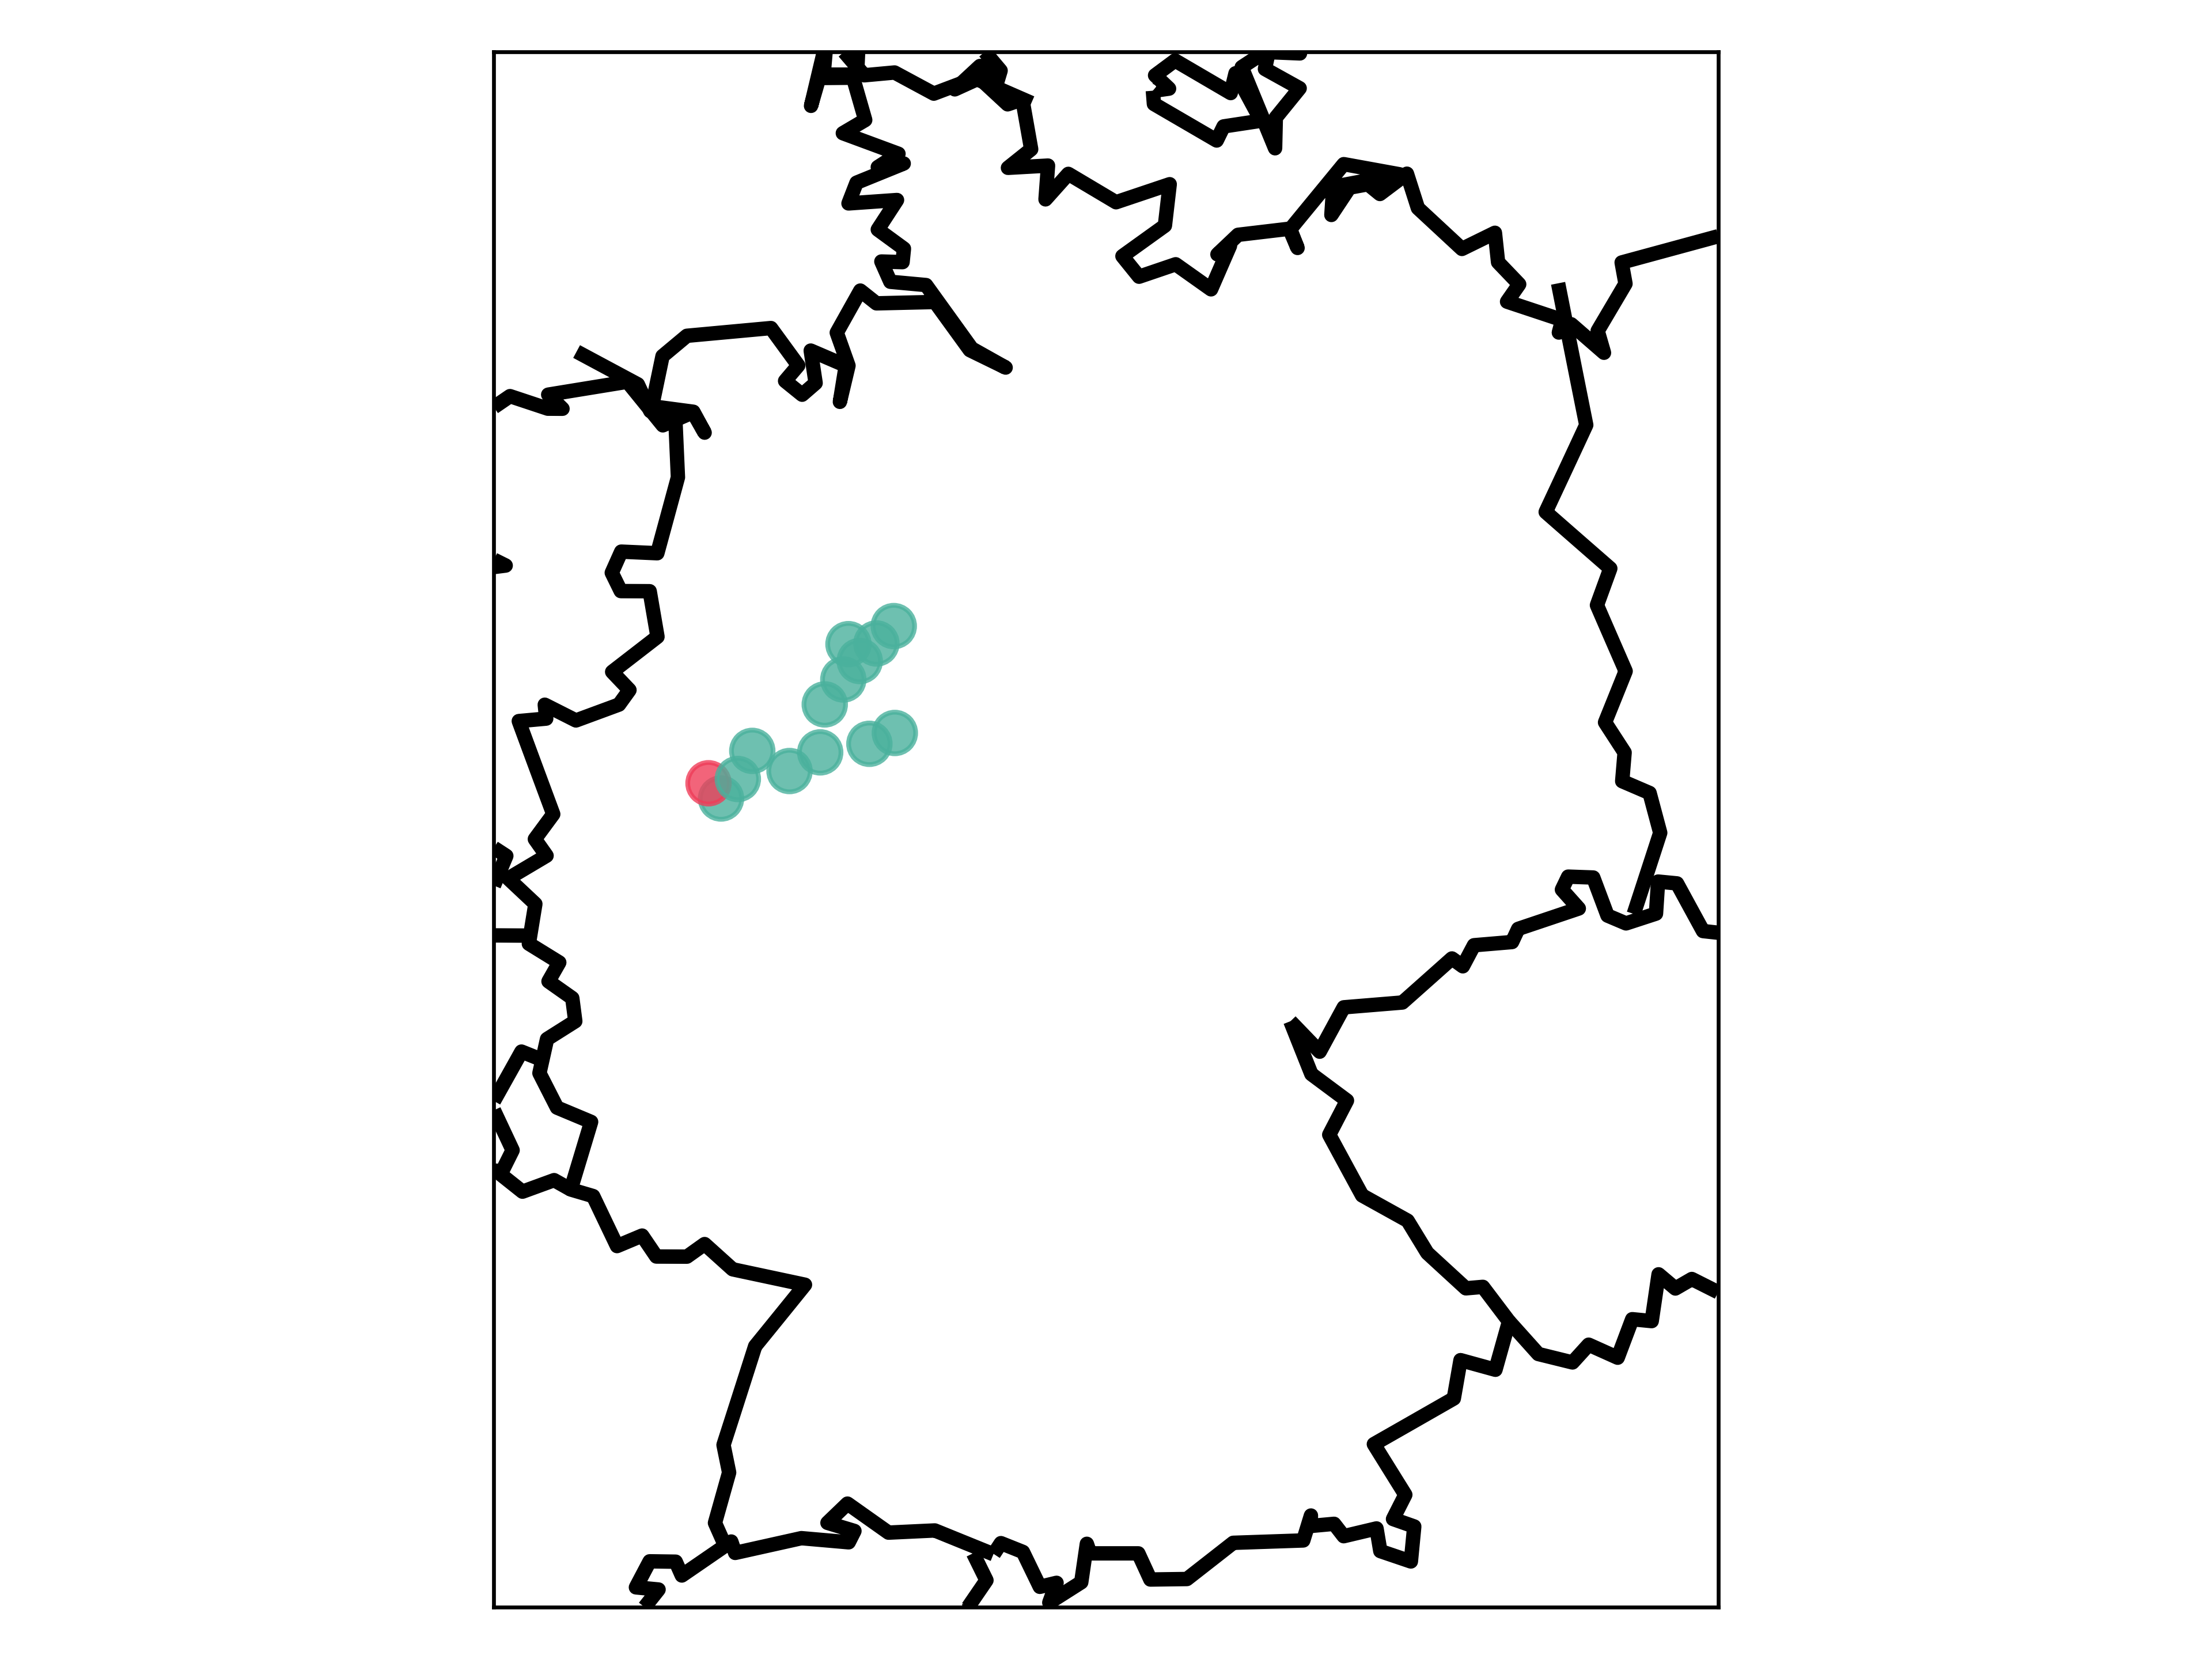
\includegraphics[clip=true,width=\columnwidth]{../data/visualizations/Dortmund_controlled_stations.png}
  \caption{Visualization of the train stations controlled by Dortmund main station, which is colored in red}
   \label{fig:do-control}
\end{figure}

Consequently, it may be more challenging to coordinate traffic among these stations with precision. 
Moreover, a significant proportion of the managed stations are situated in the north of Bavaria, at the border with other federal states. 
The aforementioned regions are overseen by other control centers, which necessitates coordination among these control centers, thereby rendering this region more challenging to control.

A linear model that incorporates all the previously introduced predictor variables also yields new insights. 
The only significant p-value indicates a positive correlation between delay and the control center at Dortmund main station. 
As illustrated in Figure~\ref{fig:do-control}, the region managed stations are in close proximity to one another, making them more susceptible to delays. 
This phenomenon is the inverse of that observed at the Nürnberg main station.

\maketitle
\section{\label{sec:Discussion}Discussion}

The experiments conducted have led to the identification of various factors influencing the delay of the German railway service. 
Of particular interest is the observation that certain operators are able to maintain a low delay at their stations, despite the high number of stations they are responsible for. 
This provides a valuable insight into the potential for reducing the overall delay across the network, as the methods employed by the operator \textit{Nahverkehrsgesellschaft-Baden-Württemberg-MBH} can be studied and applied to other parts of the network. 

Given that the operator with a negative influence on delay did not have a significant number of stations to manage, it may be a potential solution to reduce the size of some operating region in order to mitigate the impact of delay. 

Furthermore, the experiments yielded the discovery of specific control centres that exhibited a positive correlation with delay, namely Dortmund Main Station and Nuremberg Main Station. 
One possible reason for this phenomenon was the geographic distance between the control centres. In contrast, the stations in Dortmund are situated in close proximity, which facilitates the propagation of delay effects. 
The railway stations under the control of Nürnberg are distributed over a considerable area, which makes it more challenging to anticipate potential train movements. 
This is due to the fact that there is more room for maintenance on the train tracks, which in turn can result in trains departing at a later time in order to avoid track congestion. 

Finally, the centrality measures and other metadata demonstrated a positive correlation between the size of a station and its average delay, as well as its standard deviation. 
This phenomenon can be explained by the fact that the greater the number of trains that must be managed, the more challenging it is to adhere to all time constraints. 
For instance, long-distance trains may depart at a later time, as they must wait for connecting trains that are not on time.

However, the accuracy of the results is limited by the amount of data used. Since only two months of timetable data was considered, it would be a possible idea for future research to include data of a larger timespan. 
It may also be helpful to consider external events, such as holidays, or particular circumstances, as the number of trains handled by a train station also indicated a slight positive relationship with average delay.

\maketitle
\section{\label{sec:Conclusion}Conclusion}

In this paper in linear regression models have been used in order to determine possible reasons for train delay based on centrality measures and additional collected metadata about train stations. 

The most significant and unexpected outcome was the ability of this method to identify specific operators and control centers with either a positive or negative correlation to average delay, despite the models not providing this information for all operators and control centers. 
This would represent a potential starting point for future research, where additional data, such as delay data over an extended period of time, or for example weather and railway employee movement data, could be utilized to yield more interesting results. 

Nevertheless, the current results are beneficial in directing spending towards potential areas for improvement in order to enhance the overall network reliability, thereby making commuting by train a more attractive proposition.
\pagebreak
\listoffigures
\listoftables
\printbibliography

\end{document}